\documentclass{standalone}
\usepackage{tikz}
\usetikzlibrary{patterns, positioning}

\begin{document}
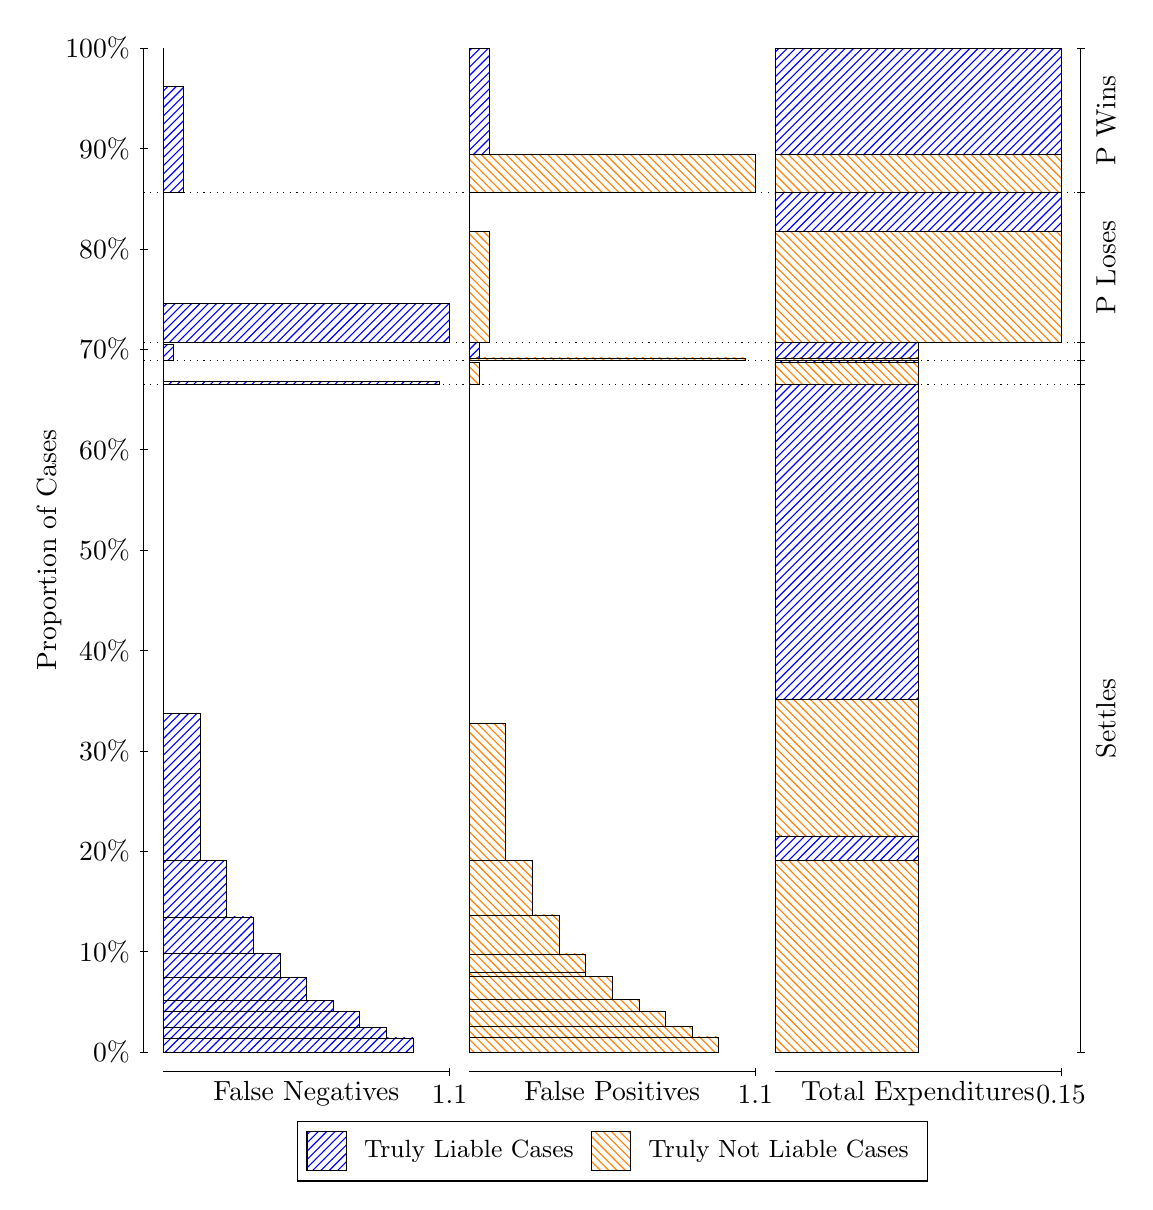
\begin{tikzpicture}
\draw[black, very thin] (1.5,1.75) -- (1.5,14.5);
\node[rotate=90, anchor=center] at (0.3, 8.125) {Proportion of Cases};
\draw[black, very thin] (1.45,1.75) -- (1.55,1.75);
\node[anchor=east] at (1.45, 1.75) {0\%};
\draw[black, very thin] (1.45,3.025) -- (1.55,3.025);
\node[anchor=east] at (1.45, 3.025) {10\%};
\draw[black, very thin] (1.45,4.3) -- (1.55,4.3);
\node[anchor=east] at (1.45, 4.3) {20\%};
\draw[black, very thin] (1.45,5.575) -- (1.55,5.575);
\node[anchor=east] at (1.45, 5.575) {30\%};
\draw[black, very thin] (1.45,6.85) -- (1.55,6.85);
\node[anchor=east] at (1.45, 6.85) {40\%};
\draw[black, very thin] (1.45,8.125) -- (1.55,8.125);
\node[anchor=east] at (1.45, 8.125) {50\%};
\draw[black, very thin] (1.45,9.4) -- (1.55,9.4);
\node[anchor=east] at (1.45, 9.4) {60\%};
\draw[black, very thin] (1.45,10.675) -- (1.55,10.675);
\node[anchor=east] at (1.45, 10.675) {70\%};
\draw[black, very thin] (1.45,11.95) -- (1.55,11.95);
\node[anchor=east] at (1.45, 11.95) {80\%};
\draw[black, very thin] (1.45,13.225) -- (1.55,13.225);
\node[anchor=east] at (1.45, 13.225) {90\%};
\draw[black, very thin] (1.45,14.5) -- (1.55,14.5);
\node[anchor=east] at (1.45, 14.5) {100\%};

\draw[black, very thin] (13.4,1.75) -- (13.4,14.5);
\draw[black, very thin] (13.35,1.75) -- (13.45,1.75);
\node[anchor=west] at (13.35, 1.75) {};
\draw[black, very thin] (13.35,10.229) -- (13.45,10.229);
\node[anchor=west] at (13.35, 10.229) {};
\draw[black, very thin] (13.35,10.537) -- (13.45,10.537);
\node[anchor=west] at (13.35, 10.537) {};
\draw[black, very thin] (13.35,10.764) -- (13.45,10.764);
\node[anchor=west] at (13.35, 10.764) {};
\draw[black, very thin] (13.35,12.664) -- (13.45,12.664);
\node[anchor=west] at (13.35, 12.664) {};
\draw[black, very thin] (13.35,14.5) -- (13.45,14.5);
\node[anchor=west] at (13.35, 14.5) {};

\draw[black, very thin, pattern color=blue, pattern=north east lines] (1.75,1.75) rectangle (4.9186,1.9292);
\draw[black, very thin, pattern color=blue, pattern=north east lines] (1.75,1.9292) rectangle (4.5806,2.0617);
\draw[black, very thin, pattern color=blue, pattern=north east lines] (1.75,2.0617) rectangle (4.2426,2.2615);
\draw[black, very thin, pattern color=blue, pattern=north east lines] (1.75,2.2615) rectangle (3.9047,2.4009);
\draw[black, very thin, pattern color=blue, pattern=north east lines] (1.75,2.4009) rectangle (3.5667,2.6924);
\draw[black, very thin, pattern color=blue, pattern=north east lines] (1.75,2.6924) rectangle (3.2287,3.0023);
\draw[black, very thin, pattern color=blue, pattern=north east lines] (1.75,3.0023) rectangle (2.8907,3.4643);
\draw[black, very thin, pattern color=blue, pattern=north east lines] (1.75,3.4643) rectangle (2.5527,4.1785);
\draw[black, very thin, pattern color=blue, pattern=north east lines] (1.75,4.1785) rectangle (2.2147,6.0548);
\draw[black, very thin, pattern color=orange, pattern=north west lines] (1.75,6.0548) rectangle (1.75,10.229);
\draw[black, very thin, pattern color=blue, pattern=north east lines] (1.75,10.229) rectangle (5.2566,10.262);
\draw[black, very thin, pattern color=orange, pattern=north west lines] (1.75,10.262) rectangle (1.75,10.537);
\draw[black, very thin, pattern color=blue, pattern=north east lines] (1.75,10.537) rectangle (1.8767,10.737);
\draw[black, very thin, pattern color=orange, pattern=north west lines] (1.75,10.737) rectangle (1.75,10.764);
\draw[black, very thin, pattern color=blue, pattern=north east lines] (1.75,10.764) rectangle (5.3833,11.254);
\draw[black, very thin, pattern color=orange, pattern=north west lines] (1.75,11.254) rectangle (1.75,12.664);
\draw[black, very thin, pattern color=blue, pattern=north east lines] (1.75,12.664) rectangle (2.0035,14.011);
\draw[black, very thin, pattern color=orange, pattern=north west lines] (1.75,14.011) rectangle (1.75,14.5);
\draw[black, very thin, pattern color=orange, pattern=north west lines] (5.6333,1.75) rectangle (8.8019,1.9424);
\draw[black, very thin, pattern color=orange, pattern=north west lines] (5.6333,1.9424) rectangle (8.464,2.0775);
\draw[black, very thin, pattern color=orange, pattern=north west lines] (5.6333,2.0775) rectangle (8.126,2.2666);
\draw[black, very thin, pattern color=orange, pattern=north west lines] (5.6333,2.2666) rectangle (7.788,2.4169);
\draw[black, very thin, pattern color=orange, pattern=north west lines] (5.6333,2.4169) rectangle (7.45,2.7089);
\draw[black, very thin, pattern color=orange, pattern=north west lines] (5.6333,2.7089) rectangle (7.112,2.7665);
\draw[black, very thin, pattern color=orange, pattern=north west lines] (5.6333,2.7665) rectangle (7.112,2.9944);
\draw[black, very thin, pattern color=orange, pattern=north west lines] (5.6333,2.9944) rectangle (6.774,3.49);
\draw[black, very thin, pattern color=orange, pattern=north west lines] (5.6333,3.49) rectangle (6.436,4.1841);
\draw[black, very thin, pattern color=orange, pattern=north west lines] (5.6333,4.1841) rectangle (6.0981,5.9238);
\draw[black, very thin, pattern color=blue, pattern=north east lines] (5.6333,5.9238) rectangle (5.6333,10.229);
\draw[black, very thin, pattern color=orange, pattern=north west lines] (5.6333,10.229) rectangle (5.7601,10.503);
\draw[black, very thin, pattern color=blue, pattern=north east lines] (5.6333,10.503) rectangle (5.6333,10.537);
\draw[black, very thin, pattern color=orange, pattern=north west lines] (5.6333,10.537) rectangle (9.1399,10.564);
\draw[black, very thin, pattern color=blue, pattern=north east lines] (5.6333,10.564) rectangle (5.7601,10.764);
\draw[black, very thin, pattern color=orange, pattern=north west lines] (5.6333,10.764) rectangle (5.8868,12.175);
\draw[black, very thin, pattern color=blue, pattern=north east lines] (5.6333,12.175) rectangle (5.6333,12.664);
\draw[black, very thin, pattern color=orange, pattern=north west lines] (5.6333,12.664) rectangle (9.2667,13.153);
\draw[black, very thin, pattern color=blue, pattern=north east lines] (5.6333,13.153) rectangle (5.8868,14.5);
\draw[black, very thin, pattern color=orange, pattern=north west lines] (9.5167,1.75) rectangle (11.333,4.1839);
\draw[black, very thin, pattern color=blue, pattern=north east lines] (9.5167,4.1839) rectangle (11.333,4.4956);
\draw[black, very thin, pattern color=orange, pattern=north west lines] (9.5167,4.4956) rectangle (11.333,6.2356);
\draw[black, very thin, pattern color=blue, pattern=north east lines] (9.5167,6.2356) rectangle (11.333,10.229);
\draw[black, very thin, pattern color=orange, pattern=north west lines] (9.5167,10.229) rectangle (11.333,10.503);
\draw[black, very thin, pattern color=blue, pattern=north east lines] (9.5167,10.503) rectangle (11.333,10.537);
\draw[black, very thin, pattern color=orange, pattern=north west lines] (9.5167,10.537) rectangle (11.333,10.564);
\draw[black, very thin, pattern color=blue, pattern=north east lines] (9.5167,10.564) rectangle (11.333,10.764);
\draw[black, very thin, pattern color=orange, pattern=north west lines] (9.5167,10.764) rectangle (13.15,12.175);
\draw[black, very thin, pattern color=blue, pattern=north east lines] (9.5167,12.175) rectangle (13.15,12.664);
\draw[black, very thin, pattern color=orange, pattern=north west lines] (9.5167,12.664) rectangle (13.15,13.153);
\draw[black, very thin, pattern color=blue, pattern=north east lines] (9.5167,13.153) rectangle (13.15,14.5);
\draw[black, dotted] (1.5,10.229) -- (13.4,10.229);
\draw[black, dotted] (1.5,10.537) -- (13.4,10.537);
\draw[black, dotted] (1.5,10.764) -- (13.4,10.764);
\draw[black, dotted] (1.5,12.664) -- (13.4,12.664);
\draw[black, very thin] (1.75,1.5) -- (5.3833,1.5);
\node[anchor=north] at (3.5667, 1.5) {False Negatives};
\draw[black, very thin] (5.3833,1.45) -- (5.3833,1.55);
\node[anchor=north] at (5.3833, 1.45) {1.1};

\draw[black, very thin] (5.6333,1.5) -- (9.2667,1.5);
\node[anchor=north] at (7.45, 1.5) {False Positives};
\draw[black, very thin] (9.2667,1.45) -- (9.2667,1.55);
\node[anchor=north] at (9.2667, 1.45) {1.1};

\draw[black, very thin] (9.5167,1.5) -- (13.15,1.5);
\node[anchor=north] at (11.333, 1.5) {Total Expenditures};
\draw[black, very thin] (13.15,1.45) -- (13.15,1.55);
\node[anchor=north] at (13.15, 1.45) {0.15};

\node[black, centered, rotate=90] at (13.72, 5.9893) {Settles};


\node[black, centered, rotate=90] at (13.72, 11.714) {P Loses};
\node[black, centered, rotate=90] at (13.72, 13.582) {P Wins};

\draw (7.449999999999999,1.5) node[draw=none] (baseCoordinate) {};
\begin{scope}[align=center]
        \matrix[scale=0.5, draw=black, below=0.5cm of baseCoordinate, nodes={draw}, column sep=0.1cm]{
            \node[rectangle, draw, minimum width=0.5cm, minimum height=0.5cm, pattern=north east lines, pattern color=blue] {}; &
            \node[draw=none, font=\small] (B) {Truly Liable Cases}; &
            \node[rectangle, draw, minimum width=0.5cm, minimum height=0.5cm, pattern=north west lines, pattern color=orange] {}; &
            \node[draw=none, font=\small] (B) {Truly Not Liable Cases}; \\
            };
\end{scope}

\end{tikzpicture}
\end{document}